\documentclass[runningheads]{llncs}

\usepackage[T1]{fontenc}
\usepackage{amsmath,amssymb,amsfonts}
\usepackage{algorithmic}
\usepackage{graphicx}
\usepackage{xcolor}
\usepackage{booktabs}
\usepackage{url}
\usepackage{array}

\newcolumntype{L}[1]{>{\raggedright\arraybackslash}p{#1}}

\begin{document}

\title{A Drift-Aware MLOps Framework for Multi-Model Serving: A Network Intrusion Detection Case Study}

\titlerunning{A Drift-Aware MLOps Framework for Multi-Model Serving}

\author{Hoang Tran-Nguyen-Viet\inst{1} \and
Thai Bui-Ngoc\inst{1} \and
Tuan Le-Anh\inst{1} \and
Bao Nguyen-Van\inst{1} \and
Quan Le-Trung\inst{1}
}

\authorrunning{Hoang Tran-Nguyen-Viet et al.}

\institute{Faculty of Computer Networks and Communications,\\
University of Information Technology, VNU-HCM,\\Ho Chi Minh City, Vietnam\\
\email{\{23520541,23521412\}@gm.uit.edu.vn, \{tuanla,baonv,quanlt\}@uit.edu.vn}}

\maketitle

\begin{abstract}
Machine learning systems deployed in production can degrade when data distributions change, even if source code remains unchanged. This issue is critical for network intrusion detection, where traffic and attack behavior evolve over time. This paper does not propose a new intrusion detection classifier; instead, it presents a baseline drift-aware MLOps framework for user-imported and training-job-created tabular models, using Network Intrusion Detection Systems (NIDS) as a case study. The framework separates model governance from model serving through a control-plane/data-plane architecture and formalizes the lifecycle over tenants, models, inference requests, production windows, drift scores, and lifecycle actions. The prototype uses Django/FastAPI services, PostgreSQL, Redpanda, Kubernetes-native training through Argo Workflows and Kubeflow PyTorchJob resources, S3-compatible object storage, optional MLflow support, and Evidently AI. It demonstrates how model artifacts can be onboarded, registered in a native model-evolution registry, served as APIs, monitored from production logs, and evaluated for Data Drift.

\keywords{MLOps \and Data Drift \and Multi-model Serving \and Model Monitoring \and Network Intrusion Detection}
\end{abstract}

\section{Introduction}

Machine learning (ML) models are increasingly deployed as continuously running services rather than offline experimental artifacts. In a production setting, a model receives new input samples over time, generates predictions for downstream users or systems, and depends on monitoring mechanisms to remain trustworthy. Unlike traditional software services, an ML service may degrade even when its source code and infrastructure remain unchanged. One major cause is Data Drift, where the production data distribution differs from the reference distribution used during training, validation, or initial deployment.

This problem is especially relevant in Network Intrusion Detection Systems (NIDS). Network traffic is non-stationary: benign usage patterns change, infrastructure evolves, and attack strategies continuously adapt. A classifier trained on historical flow features may therefore become less reliable when deployed in a new environment or under a new attack distribution. An operational NIDS should not only expose a prediction API but also record production data, compare it with reference data, and trigger lifecycle actions when the monitored distribution changes.

Existing MLOps research provides architectural concepts for automating ML development, deployment, and monitoring \cite{kreuzberger2023mlops}. Other works discuss MLOps maturity, pipeline platforms, data quality, and continual model maintenance \cite{john2021towards,subramanya2022devops,renggli2021data}. However, practical systems often treat monitoring as a passive observability layer. In many prototypes, drift reports are generated after deployment, but the monitoring result is not explicitly modeled as a control signal for model lifecycle decisions.

This paper presents a baseline framework that connects multi-model serving with drift-aware monitoring. The goal is to describe a reusable MLOps framework, not to claim a new state-of-the-art NIDS classifier. In the proposed design, NIDS is used as a case study because it naturally exposes the need for drift-aware operation. The framework is intentionally scoped to tabular classification models that are either imported by users or produced by controlled training jobs and then converted into serving-compatible artifacts.

The main contributions of this paper are:

\begin{itemize}
    \item We propose a tenant-aware and drift-aware MLOps framework that integrates model onboarding, dynamic serving, production logging, drift detection, and lifecycle adaptation triggers.
    \item We formalize the framework using tenants, model functions, reference data, production windows, feature-level drift indicators, dataset-level drift ratio, and an action-selection function.
    \item We implement a prototype platform and instantiate it with a Network Intrusion Detection case study to demonstrate the feasibility of the proposed lifecycle.
\end{itemize}

The remainder of this article is structured as follows. Section~2 reviews related work on MLOps lifecycles, serving platforms, data quality, drift monitoring, and ML-based NIDS. Sections~3--5 define the problem, present the framework, and describe the drift-aware lifecycle algorithm; Sections~6--8 instantiate the framework in the NIDS case study, describe the prototype, and report preliminary evaluation results. Sections~9 and~10 discuss limitations and conclude the paper.

\section{Related Work}

\subsection{MLOps Architectures and Lifecycle}

MLOps extends DevOps principles to ML systems by coordinating data engineering, experimentation, training, deployment, monitoring, and governance. Kreuzberger \textit{et al.} define MLOps as a paradigm for reliably and efficiently developing and maintaining ML systems in production \cite{kreuzberger2023mlops}, while John \textit{et al.} propose a maturity model for assessing MLOps adoption \cite{john2021towards}. Sculley \textit{et al.} show that ML systems accumulate technical debt beyond model code, including data dependencies, configuration, monitoring, and feedback loops \cite{sculley2015debt}. Amershi \textit{et al.} further show that software engineering for ML differs from traditional software engineering because data, models, and code evolve together \cite{amershi2019software}. Our work narrows these lifecycle concerns to drift-aware signals for tenant-aware multi-model serving.

\subsection{MLOps Platforms, Model Registry, and Model Serving}

Implementation-oriented MLOps studies show how platform components connect model development and deployment. TFX integrates data ingestion, validation, training, and serving \cite{baylor2017tfx}; MLflow supports tracking and model lifecycle management \cite{mlflow}; and Clipper frames online prediction as a systems problem \cite{crankshaw2017clipper}. Earlier platform case studies discuss ML pipeline and domain workflows \cite{zhou2020pipeline,subramanya2022devops}, while recent work frames MLOps as self-adaptive architecture \cite{Bhatt2025HarmonE}. A recent empirical evaluation compares MLflow, Metaflow, Airflow, and Kubeflow Pipelines across installation, flexibility, interoperability, instrumentation, interpretability, and documentation, showing complementary strengths rather than one universal lifecycle abstraction \cite{MarcosMercade2026MLOpsFrameworks}.

\begin{table}[t]
\caption{MLOps tool-family scope and remaining gap.}
\label{tab:mlops-tool-gap}
\centering
\small
\begin{tabular}{@{}L{2.2cm}L{3.2cm}L{5.8cm}@{}}
\toprule
\textbf{Tool family} & \textbf{Main support} & \textbf{Gap relative to this work} \\
\midrule
MLflow & Tracking, artifacts, registry. & Tenant ownership, lifecycle state, serving logs, and UI actions need product control-plane logic. \\
Flow tools & Workflow orchestration. & Registry governance, multi-model serving, and drift-driven review remain external concerns. \\
Kubeflow/TFX & Pipeline and cloud-native ML workflows. & Tenant lifecycle, registry views, and drift summaries must be mapped into application metadata. \\
Proposed framework & Registry, serving, logs, drift, and artifacts under one control plane. & Baseline prototype; production hardening and autonomous promotion remain future work. \\
\bottomrule
\end{tabular}
\end{table}

\subsection{Data Quality, Data Drift, and Concept Drift Monitoring}

Production ML reliability depends on the data observed after deployment as well as on the pipelines that manage that data. Renggli \textit{et al.} argue that data quality should be treated as a first-class MLOps concern \cite{renggli2021data}, and Polyzotis \textit{et al.} identify data management challenges that arise in production ML pipelines \cite{polyzotis2017data}. Data Drift and concept drift are related but distinct concerns: Gama \textit{et al.} survey adaptation to changing data streams \cite{gama2014survey}, while Webb \textit{et al.} characterize different forms of concept drift \cite{webb2016drift}. In this paper, Data Drift is used as an operational signal. Because production labels may be delayed or unavailable, the system first compares input distributions and then triggers inspection or workflow handoff when drift is detected.

\subsection{Cybersecurity/NIDS as a Non-Stationary Case Study}

Network intrusion detection provides a useful non-stationary case study for drift-aware MLOps. CIC-IDS2017 provides labeled intrusion traffic for evaluating intrusion detection models \cite{cicids}, but real deployment environments can differ from dataset conditions. Sommer and Paxson argue that ML-based intrusion detection faces challenges outside closed-world assumptions, including deployment context, generalization, and evolving traffic distributions \cite{sommer2010closedworld}. Recent NIDS research likewise treats concept drift as an operational problem requiring continual or online adaptation policies for evolving traffic patterns \cite{Zhang2025SSFNIDS}. This paper therefore uses NIDS to illustrate lifecycle and monitoring requirements, not to claim a new state-of-the-art intrusion detection classifier.

\subsection{Research Gap}

The reviewed literature covers MLOps architectures, platforms, serving, data quality, drift adaptation, and NIDS deployment challenges. Existing tools provide useful building blocks, but they often center on tracking, orchestration, or pipeline execution rather than a tenant-facing lifecycle abstraction for multi-model serving. This paper addresses that gap by placing a Native Registry in the control plane as the product-level source of truth for tenant ownership, model families, versions, deployment metadata, production-log summaries, drift results, and review-driven lifecycle actions. Existing tools remain adapters for tracking, training execution, artifact storage, and drift reporting; the contribution is the integration pattern connecting them into a drift-aware multi-tenant serving lifecycle.

\section{Problem Formulation}

Let $\mathcal{U}=\{u_1,u_2,\ldots,u_N\}$ denote the set of tenants using the platform. Each tenant $u \in \mathcal{U}$ owns a set of registered models:

\begin{equation}
\mathcal{M}_u=\{m_{u,1},m_{u,2},\ldots,m_{u,K_u}\}.
\end{equation}

Each model $m_{u,i}$ is represented by an inference function parameterized by $\theta$:

\begin{equation}
\hat{y}_t=f_{\theta}^{u,i}(x_t),
\end{equation}

where $x_t \in \mathbb{R}^{d}$ is the input vector at time $t$, $d$ is the number of input features, and $\hat{y}_t$ is the prediction. For a tabular classification model, $\hat{y}_t$ may be a class label or a probability vector over class labels.

For every inference request, the platform records a production log:

\begin{equation}
z_t=(u,i,x_t,\hat{y}_t,c_t,t),
\end{equation}

where $c_t$ is the prediction confidence if available. The log stream associated with a tenant-model pair $(u,i)$ forms the basis for monitoring.

Each deployed model has a reference dataset:

\begin{equation}
D_{\mathrm{ref}}^{u,i}=\{x_1,x_2,\ldots,x_n\},
\end{equation}

which represents the distribution observed during training, validation, or initial acceptance. At monitoring time $T$, the current production data window is:

\begin{equation}
D_{\mathrm{cur}}^{u,i}(T)=\{x_t \mid T-W \leq t \leq T\},
\end{equation}

where $W$ is the monitoring window size. The objective is not only to compute predictions but also to select a lifecycle action:

\begin{equation}
a_T = \pi(m_{u,i},D_{\mathrm{ref}}^{u,i},D_{\mathrm{cur}}^{u,i}(T),S_T),
\end{equation}

where $\pi(\cdot)$ is the adaptation policy and $S_T$ is the current lifecycle state of the model. Possible actions include no operation, alert generation, manual review, retraining trigger, and review-driven rollback or promotion candidates.

For each feature $j$, the framework computes a drift score:

\begin{equation}
\delta_j=\Delta(P_{\mathrm{ref}}(x_j),P_{\mathrm{cur}}(x_j)),
\end{equation}

where $\Delta(\cdot)$ is a statistical distance or hypothesis test between the reference and current feature distributions. A feature-level drift indicator is defined as:

\begin{equation}
I_j =
\begin{cases}
1, & \delta_j > \tau_j,\\
0, & \mathrm{otherwise},
\end{cases}
\end{equation}

where $\tau_j$ is the threshold for feature $j$. The dataset-level drift ratio is:

\begin{equation}
\rho=\frac{1}{d}\sum_{j=1}^{d}I_j.
\end{equation}

The final drift decision is:

\begin{equation}
\mathrm{Drift}(D_{\mathrm{ref}}, D_{\mathrm{cur}}) =
\begin{cases}
1, & \rho \ge \tau_D,\\
0, & \text{otherwise}.
\end{cases}
\end{equation}

where $\tau_D$ is the dataset-level threshold. This formulation separates model prediction from monitoring and makes Data Drift an explicit input to lifecycle decisions.

\section{Proposed Framework}

The logical flow of the proposed framework consists of four stages. First, a user onboards a model artifact or registers an artifact produced by a controlled training workflow through the control plane. Second, the data plane exposes the model as a prediction endpoint. Third, each prediction produces an asynchronous log event. Fourth, the monitoring layer periodically reconstructs the current production window and compares it with the reference data. If drift is detected, the adaptation layer creates an alert or triggers a retraining workflow.

% TODO: Add system architecture overview figure showing Web/User, Django/DRF Control Plane, Kubeflow training workflow or Kubernetes training resource, training pods, Karpenter NodePool/NodeClaim boundary where configured, Object Storage, Native Registry/PostgreSQL, FastAPI Model Server, Redpanda/Consumer, Evidently Drift Monitoring, and deployment boundary.
% TODO: Add prototype screenshots only if page count remains within the 14-page limit.
% Candidate screenshots: training job detail, Model Evolution, drift report, CI/CD run, Kubernetes/Karpenter status, Kubeflow/Argo training run status, and artifact/registry ingest evidence.

\subsection{Control Plane}

The control plane manages user-facing and governance operations. It stores tenants, authentication credentials, API keys, model metadata, artifact locations, endpoint URLs, access modes, and model statuses. In the prototype, this layer is implemented using Django. A model record contains the model name, description, owner tenant, artifact URI, access mode, generated endpoint, and lifecycle status.

When a model artifact is uploaded or registered from a completed training job, the control plane validates the available metadata, stores artifact references, and records the model in the native registry. The model can then be assigned an endpoint of the form \texttt{/models/\{model\_id\}/predict}. This design decouples model ownership and metadata management from online inference.

\subsection{Data Plane}

The data plane is implemented as a generic FastAPI model server. The logical serving path resolves models through a shared API, while deployment adapters may create dedicated runtime resources when configured. The server reads the corresponding model metadata, loads the model artifact through MLflow pyfunc, validates the request payload against the expected input format when possible, and returns the prediction result.

Tenant-aware access control is enforced before inference. Public models can be invoked directly, while private models require a valid API key or bearer token. The resolved tenant identifier must match the model owner. This mechanism supports a platform setting where multiple users upload and serve independent models through a shared serving layer.

\subsection{Production Logging Layer}

Online inference should not depend synchronously on database writes. Therefore, the framework decouples prediction from logging through a message broker. After producing a prediction, the model server emits a production log event to Redpanda. A consumer service batches log events and persists them to PostgreSQL. Each log stores the tenant identifier, model identifier, timestamp, feature payload, and prediction result.

This design has two advantages. First, it keeps monitoring writes outside the synchronous prediction path. Second, it creates a unified production data source that can be queried per tenant and per model for drift detection, audit, and evaluation.

\subsection{Drift Monitoring Layer}

The monitoring layer compares reference data with recent production data. In the prototype, Evidently AI is used to compute feature-level drift and dataset-level drift summaries. Reference data can be stored as object storage artifacts, while production data are reconstructed from PostgreSQL logs. Drift reports can be exported as HTML or JSON artifacts for inspection.

\subsection{Adaptation Layer}

The adaptation layer maps monitoring outputs to lifecycle actions. In the baseline implementation, the primary action is a drift alert or workflow trigger. The framework can be extended to support retraining jobs, model evaluation gates, review-driven promotion, rollback, and notification workflows. This distinction is important: the current prototype demonstrates a drift-aware control loop, while fully autonomous retraining and deployment remain future work.

\section{Drift-Aware Lifecycle Algorithm}

The model lifecycle can be represented as a state transition system:

\begin{equation}
\begin{split}
S \in \{&
\mathrm{uploaded},\ \mathrm{validated},\ \mathrm{deployed},\
\mathrm{monitored},\\
&\mathrm{drifted},\ \mathrm{reviewing},\ \mathrm{retraining},\
\mathrm{promoted},\ \mathrm{failed}
\}.
\end{split}
\end{equation}

The transition function is:

\begin{equation}
S_{T+1}=\Phi(S_T,m_{u,i},\rho,\tau_D,a_T),
\end{equation}

where $\Phi(\cdot)$ updates the model state according to the drift ratio and the selected action. If $\rho < \tau_D$, the model remains in the monitored state. If $\rho \geq \tau_D$, the model is marked as drifted and the system can trigger alerting, review, or a workflow handoff.

\begin{figure}[t]
\small
\begin{algorithmic}[1]
\REQUIRE Model package or training artifact $A$, metadata $H$, tenant $u$
\ENSURE Registered model endpoint $e$
\STATE Validate package extension and archive structure
\STATE Validate serving metadata or record deployability status
\STATE Store or reference $A$ in artifact storage
\STATE Create model record $m_{u,i}$ in the control plane
\STATE Assign lifecycle state $S \leftarrow \mathrm{validated}$
\STATE Generate endpoint $e \leftarrow$ \texttt{/models/\{i\}/predict}
\STATE Return endpoint $e$
\end{algorithmic}
\caption{Model onboarding procedure.}
\label{alg:onboarding}
\end{figure}

\begin{figure}[t]
\small
\begin{algorithmic}[1]
\REQUIRE Input $x_t$, model identifier $i$, credential $q$
\ENSURE Prediction $\hat{y}_t$ and optional lifecycle action $a_T$
\STATE Authenticate $q$ and resolve tenant $u$
\STATE Retrieve model metadata $m_{u,i}$
\STATE Load or reuse cached model $f_{\theta}^{u,i}$
\STATE Compute prediction $\hat{y}_t \leftarrow f_{\theta}^{u,i}(x_t)$
\STATE Emit log event $z_t=(u,i,x_t,\hat{y}_t,t)$
\IF{monitoring condition is satisfied}
    \STATE Build production window $D_{\mathrm{cur}}^{u,i}(T)$
    \FOR{each feature $j=1$ to $d$}
        \STATE Compute drift score $\delta_j$
        \STATE Compute indicator $I_j$
    \ENDFOR
    \STATE Compute drift ratio $\rho$
    \STATE Select action $a_T \leftarrow \pi(m_{u,i},D_{\mathrm{ref}},D_{\mathrm{cur}},S_T)$
    \IF{$\rho \geq \tau_D$}
        \STATE Trigger alert, review, or workflow handoff
    \ENDIF
\ENDIF
\STATE Return $\hat{y}_t$
\end{algorithmic}
\caption{Drift-aware inference and monitoring procedure.}
\label{alg:monitoring}
\end{figure}

\section{Case Study: Network Intrusion Detection}

The NIDS model is used as a case study to instantiate the proposed framework. A network flow is represented as a tabular feature vector $x \in \mathbb{R}^{d}$ containing statistics such as duration, packet counts, byte rates, and protocol-related attributes. The model predicts whether the observed traffic is benign or belongs to an attack class.

In the current prototype, XGBoost is selected as the baseline classifier rather than as a claim of state-of-the-art NIDS performance. The case study uses tabular network-flow features, where tree-based gradient boosting provides a practical balance between non-linear feature interaction modeling, training cost, inference efficiency, and artifact portability \cite{xgboost}. Compared with simple linear baselines, XGBoost can capture interactions among flow statistics such as duration, packet counts, and byte rates. Compared with deep neural models, it requires less task-specific architecture design and is easier to package, version, and serve as a compact artifact in a multi-tenant MLOps prototype. Therefore, XGBoost is used to exercise the lifecycle--training, packaging, registration, endpoint invocation, production logging, and drift monitoring--rather than to optimize NIDS classification accuracy. Other classifiers can be onboarded through the same artifact and registry workflow when they satisfy the serving contract.

NIDS is an appropriate case study for drift-aware MLOps for three reasons. First, network environments change over time, causing benign traffic distributions to shift. Second, attack patterns evolve, making historical training data incomplete. Third, labeled production data are often delayed or unavailable, so input distribution monitoring can provide an early warning signal before supervised performance metrics are available.

\section{Prototype Implementation}

This section describes the implemented prototype as reflected in the repository. The purpose is to document the system boundary and implementation coverage, not to claim production readiness or performance characteristics.

\subsection{Prototype Architecture}

The prototype follows a control-plane/data-plane architecture. The control plane is implemented with Django and Django REST Framework and stores users, tenants, training jobs, model API records, registry versions, deployment metadata, and drift monitoring records in PostgreSQL. The data plane is implemented as a FastAPI model server that resolves a model endpoint, loads the serving artifact, performs prediction, and emits production log events. Redpanda is used as the asynchronous log transport, and a consumer service persists prediction records into PostgreSQL for later drift analysis.

Figure~\ref{fig:prototype-flow} summarizes the implemented prototype workflow across the control plane, data plane, training execution, artifact storage, production logging, and drift monitoring components.

\begin{figure}[t]
\centering
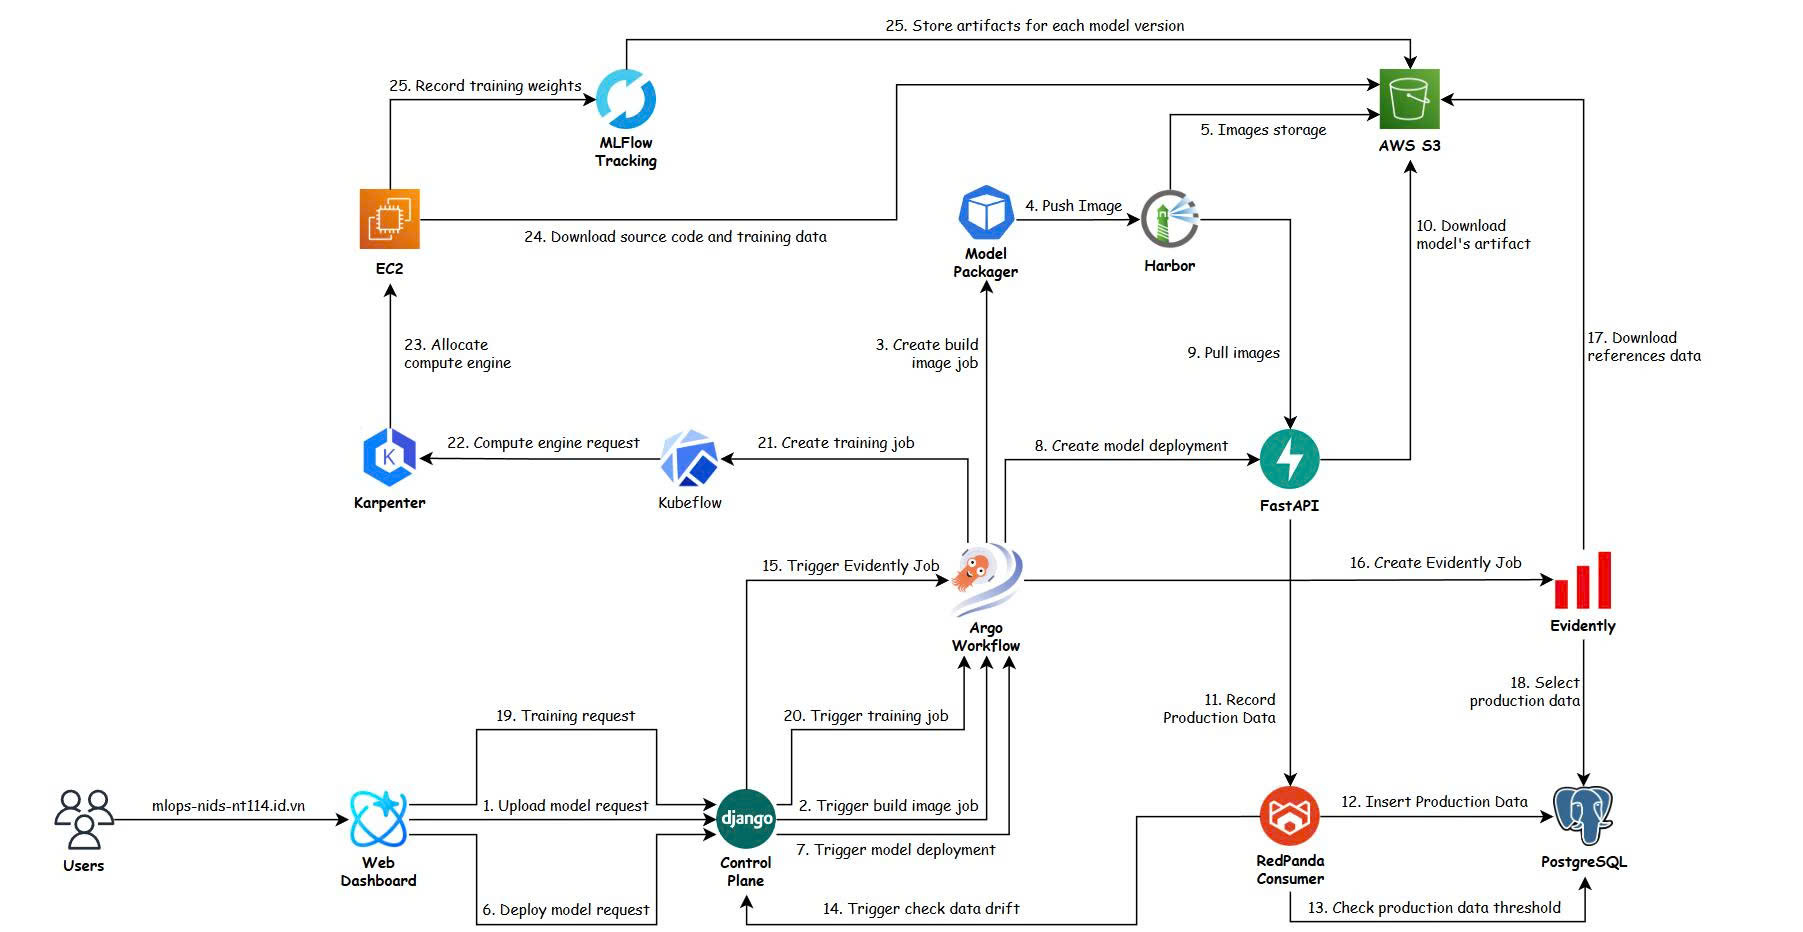
\includegraphics[width=\linewidth]{assets/flow.png}
\caption{Prototype workflow of the drift-aware MLOps framework. The Django control plane coordinates upload, packaging, training requests, deployment requests, registry metadata, and drift checks. The FastAPI data plane serves model predictions and emits production logs through Redpanda/PostgreSQL, while Argo/Kubeflow, object storage, Harbor, MLflow, Evidently, and Karpenter-backed compute are used as supporting services where configured.}
\label{fig:prototype-flow}
\end{figure}

The implementation also includes S3-compatible artifact storage, Kubernetes training workflows using Kubeflow PyTorchJob resources, a Python training runner, a model packager, MLflow integration, Evidently-based drift monitoring, and a Native Registry/Model Evolution layer. In the user-facing workflow, Native Registry data stored in PostgreSQL is the source of truth for Model Evolution. MLflow is treated as internal experiment lineage and model-format support rather than a required user interface.

\begin{table}
\caption{Prototype modules and responsibilities.}
\label{tab:implementation}
\centering
\small
\begin{tabular}{@{}L{2.6cm}L{2.8cm}L{6.0cm}@{}}
\toprule
\textbf{Module} & \textbf{Implementation} & \textbf{Responsibility} \\
\midrule
Control plane & Django/DRF & Manages tenants, jobs, registry, deployment, and drift APIs. \\
Training execution & Argo/Kubeflow + runner & Executes configured entry points and returns artifacts. \\
Artifact/registry layer & Object storage + PostgreSQL & Stores model artifacts, metadata, and version summaries. \\
Packaging/serving & Packager + FastAPI & Prepares or loads serving artifacts and exposes prediction endpoints. \\
Logging/drift & Redpanda + consumer + Evidently & Persists production logs and stores drift summaries. \\
Deployment configuration & Docker Compose/K8s/Argo files & Supports local integration and prototype/testbed deployment. \\
\bottomrule
\end{tabular}
\end{table}

\subsection{Training Job Execution}

Training jobs can be created from uploaded source packages or code stored through the Source Editor workflow. In the Kubernetes-native path, the control plane validates the selected source and reference data, prepares S3-compatible references and presigned URLs, and sends a training request to Argo Events. Argo Workflows instantiate a Kubeflow \texttt{PyTorchJob} in the training namespace, where the runner executes the configured entry point and uploads the resulting \texttt{model.tar.gz} artifact to object storage.

The non-local path does not require user scripts to import MLflow or receive MLflow credentials. User scripts write model artifacts and optional metadata; the runner packages the output, and a completion webhook updates the \texttt{TrainingJob} record so the control plane can ingest metadata and synchronize Native Registry records when the artifact is registered.

\subsection{Training Runner Output Contract}

After training completes, the runner produces a required \texttt{model.tar.gz} archive and, when available, an \texttt{\_mlops} metadata bundle containing training summary, metrics, parameters, model insights, artifact manifest, stdout/stderr logs, and warnings. Only the archive is required; the remaining metadata improves registry display and version comparison but does not invalidate the artifact when absent.

\subsection{Metadata Ingestion and Native Registry}

When a completed job is ingested, the control plane downloads the artifact, extracts metadata, and stores metrics, parameters, insights, manifest, and deployability summaries. These summaries are mirrored into Model Evolution when a model is registered from the job.

The Native Registry groups versions through family and version records linked to deployable \texttt{ModelAPI} records. Model Evolution displays tracking status, metrics, artifacts, deployability state, version comparison, deployment actions, drift summaries, and basic routing aliases.

The Native Registry is a product-level control-plane abstraction, not a replacement for existing MLOps platforms. Tenant ownership, access rules, lifecycle states, deployment aliases, drift summaries, and UI actions remain in PostgreSQL through tenant-scoped records, while Argo/Kubeflow, object storage, MLflow, and Evidently act as adapters. This separation lets imported artifacts and training-job artifacts enter one lifecycle with per-tenant ownership, version comparison, deployability review, drift-aware status, and deployment actions.

\subsection{Model Packaging and Serving}

The prototype includes a model packager that prepares serving-compatible packages or images for supported artifacts. Build execution can be triggered through a local Docker path or through an Argo-oriented workflow path, depending on deployment configuration. The FastAPI model server loads the model artifact, including MLflow pyfunc artifacts where available, and exposes generated prediction endpoints. Prediction requests can be public or private depending on model configuration and are logged asynchronously for monitoring. Serving measurements in this paper are treated as prototype observations rather than production service-level claims.

\subsection{Drift Monitoring}

Drift monitoring uses production records stored in PostgreSQL and reference data associated with a model. The Evidently integration computes feature-level and dataset-level drift summaries and stores report locations and drift result metadata in the control plane. The drift result can be exposed as a report link or summarized in Model Evolution.

In this baseline, drift is a monitoring and adaptation signal. It does not automatically redeploy a model, perform rollback, or select traffic weights. Such decisions require evaluation gates and human review policies that are outside the current baseline.

\subsection{MLflow Tracking Integration}

MLflow is used as optional internal tracking. After the control plane ingests the training artifact, it may log metrics, parameters, and metadata artifacts to an MLflow tracking server and store the run identifier. If MLflow tracking is disabled, Model Evolution still displays metrics, parameters, artifacts, model insights, and deployability information from the Native Registry. If MLflow logging fails, the metadata retained in PostgreSQL remains available for review and deployment decisions.

This design avoids requiring user training scripts to import MLflow. It also avoids making the MLflow UI the primary product workflow. The user-facing Model Evolution pages are backed by Native Registry records.

\subsection{Deployment and Operational Scope}

The repository contains Docker Compose, Kubernetes/K3s-oriented manifests, Argo workflow templates, CI/CD configuration, and GitOps-style deployment configuration updates. These assets document prototype/testbed automation rather than production hardening or evidence of latest workflow success.

Operationally, the frontend calls the Django/DRF control plane for model upload, training, registry, deployment, and drift views. The control plane exchanges artifacts with S3-compatible storage, submits training requests to Argo Events, receives callbacks after Kubeflow \texttt{PyTorchJob} execution, ingests runner artifacts into the Native Registry, receives production logs through Redpanda/PostgreSQL, and stores drift summaries. Where Karpenter is configured, training pods can match AWS-backed training node pools, but workflow logs, pod status, artifact uploads, registry ingest records, and Karpenter events should be attached separately before stronger operational claims.

The implemented baseline covers authentication, upload, Kubernetes-native training, metadata ingestion, Model Evolution, version comparison, build, deploy, and smoke-test actions, production logging, drift reports, and a basic routing alias. Autonomous retraining, automated promotion, canary or blue-green deployment, weighted traffic routing, billing, and production-grade hardening remain outside the completed baseline.

\section{Preliminary Evaluation}

Because this paper is a baseline, evaluation focuses on prototype feasibility and drift-aware lifecycle behavior rather than optimizing NIDS accuracy. We run an offline replay/recovery experiment on CIC-IDS2017-style flow data in the binary BENIGN-vs-ATTACK setting. For each attack family, a drift window is split into a trigger/retraining subset and a future holdout subset. The framework-assisted path treats the drift decision as an alert that initiates review-driven challenger training and registration; it does not bypass review gates. Row-hash checks exclude future-holdout rows from retraining. Table~\ref{tab:drift-recovery} compares the fixed XGBoost baseline with the review-driven retrained challenger.

\begin{table}[htbp]
\centering
\caption{Offline drift/retraining recovery results. Acc., M-F1, and W-F1 denote Accuracy, Macro-F1, and Weighted-F1.}
\label{tab:drift-recovery}
\small
\begin{tabular}{@{}lllll@{}}
\toprule
Scenario & Drift & Fixed Acc./M-F1/W-F1 & Retrained Acc./M-F1/W-F1 & $\Delta$M-F1 \\
\midrule
PortScan & 0.981 & 0.193 / 0.162 / 0.062 & 1.000 / 1.000 / 1.000 & +0.838 \\
BruteForce & 0.981 & 0.595 / 0.374 / 0.444 & 1.000 / 0.999 / 1.000 & +0.625 \\
WebAttacks & 0.981 & 0.874 / 0.466 / 0.816 & 0.999 / 0.997 / 0.999 & +0.531 \\
\bottomrule
\end{tabular}
\end{table}

All three scenarios exceed the drift-share threshold with 51 of 52 features marked as drifted. The retrained challengers recover Macro-F1 on future holdout windows under this offline protocol, while the result remains a prototype recovery measurement rather than evidence of direct production rollout.

We also ran a short serving benchmark against a deployed endpoint using Locust replay traffic and Prometheus metrics scraped from the serving pod \texttt{endpoint-t-1ac7d01a-model-xn102v-b8b8c59f8-hd8jj}. The run issued 4,397 client-side prediction requests over roughly two minutes with 20 virtual users. Locust measured an average response time of 213.9 ms and p95 response time of 360 ms; its failure count corresponds to label-prediction mismatches recorded by the test script, not HTTP request failures. Prometheus reported an average server-side throughput of 44.4 requests/s, peak throughput of 79.3 requests/s, average mean handler latency of 47.1 ms, and average p95 handler latency of 331.2 ms for the \texttt{/models/\{model\_id\_str\}/predict} handler. Figure~\ref{fig:endpoint-benchmark} shows the Prometheus time series used for this observation.

\begin{figure}[t]
\centering
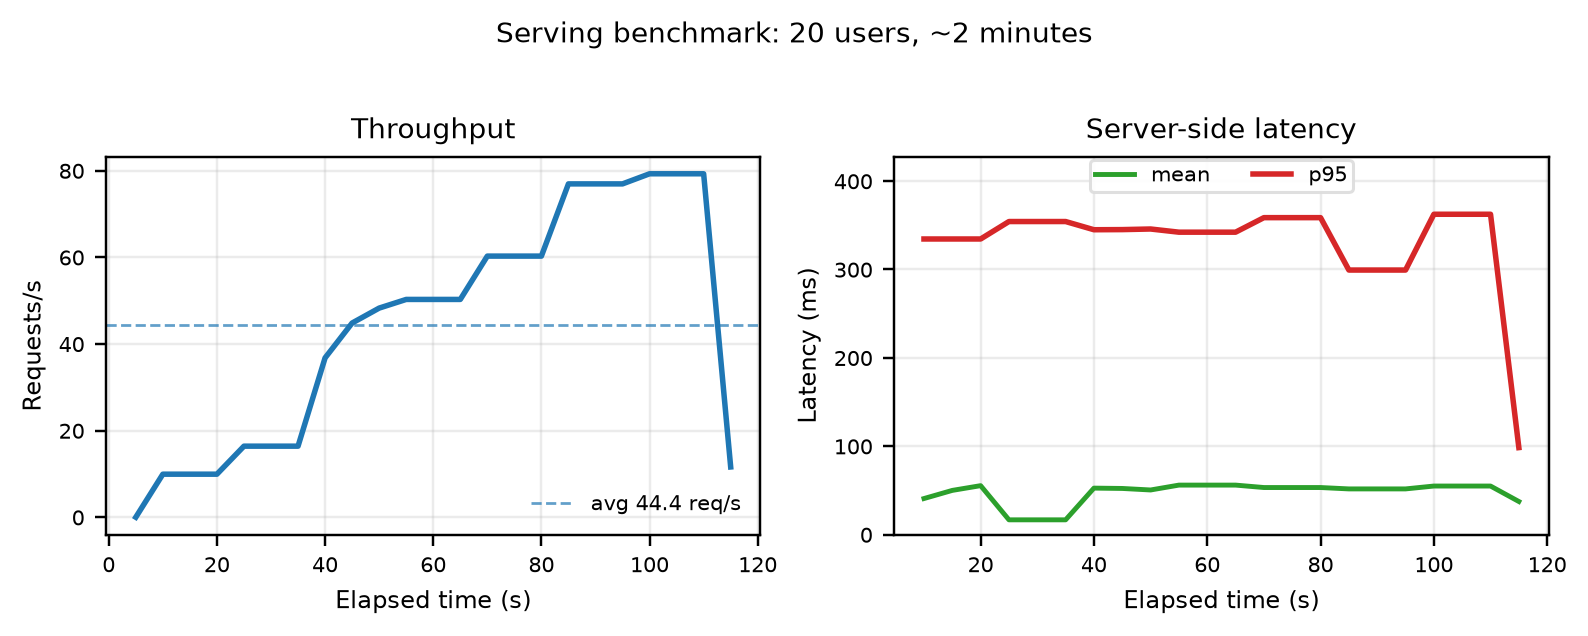
\includegraphics[width=\linewidth]{assets/chart-locust-benchmark.png}
\caption{Prototype serving benchmark with 20 Locust users over an approximately two-minute replay window. Throughput and latency are queried from Prometheus for the serving pod during the benchmark.}
\label{fig:endpoint-benchmark}
\end{figure}

\section{Discussion}

The proposed framework reframes MLOps monitoring as part of an adaptive control loop: the model server emits production evidence, and the monitoring layer produces signals that can affect lifecycle decisions. This is useful for SaaS or PaaS-style settings where different users upload different models but need a common operational pipeline.

The scope is intentionally limited. First, the system targets tabular classification artifacts; image, text, time-series, and large language models need additional schema validation and monitoring metrics. Second, arbitrary user-uploaded artifacts introduce security risks, so hardened systems must isolate execution, validate dependencies, restrict archive extraction, and enforce resource quotas. Third, autonomous retraining and promotion require reliable evaluation gates, rollback policies, and human approval. Therefore, this baseline treats drift detection as an adaptation signal rather than an unconditional redeployment decision.

\section{Conclusion}

This paper presented a baseline drift-aware MLOps framework for multi-model serving, integrating tenant-aware onboarding, Kubernetes-native training, native model-evolution metadata, dynamic endpoints, asynchronous production logging, and reference-production drift monitoring. The system was formalized using tenants, model functions, production windows, drift indicators, lifecycle states, and adaptation actions, and instantiated with Network Intrusion Detection as a non-stationary security case study. Preliminary offline recovery results show that drift alerts can support review-driven challenger retraining on future holdout windows, while future work will address artifact-execution hardening, runtime deployment evidence, evaluation gates, and additional model types.

\begin{thebibliography}{00}

\bibitem{kreuzberger2023mlops}
M. Kreuzberger, N. Kuhl, and S. Hirschl, ``Machine Learning Operations (MLOps): Overview, Definition, and Architecture,'' \textit{IEEE Access}, vol. 11, pp. 31866--31879, 2023.

\bibitem{sculley2015debt}
D. Sculley, G. Holt, D. Golovin, E. Davydov, T. Phillips, D. Ebner,
V. Chaudhary, M. Young, J.-F. Crespo, and D. Dennison,
``Hidden Technical Debt in Machine Learning Systems,''
in \textit{Advances in Neural Information Processing Systems}, vol. 28, 2015.

\bibitem{amershi2019software}
S. Amershi, A. Begel, C. Bird, R. DeLine, H. Gall, E. Kamar,
N. Nagappan, B. Nushi, and T. Zimmermann,
``Software Engineering for Machine Learning: A Case Study,''
in \textit{Proc. IEEE/ACM 41st International Conference on Software Engineering:
Software Engineering in Practice}, 2019, pp. 291--300.

\bibitem{john2021towards}
M. M. John, H. H. Olsson, and J. Bosch, ``Towards MLOps: A Framework and Maturity Model,'' in \textit{Proc. 47th Euromicro Conference on Software Engineering and Advanced Applications}, 2021, pp. 1--8.

\bibitem{zhou2020pipeline}
Y. Zhou, Y. Yu, and B. Ding, ``Towards MLOps: A Case Study of ML Pipeline Platform,'' in \textit{Proc. International Conference on Artificial Intelligence and Computer Engineering}, 2020, pp. 494--500.

\bibitem{baylor2017tfx}
D. Baylor et al.,
``TFX: A TensorFlow-Based Production-Scale Machine Learning Platform,''
in \textit{Proc. 23rd ACM SIGKDD International Conference on Knowledge Discovery and Data Mining},
2017, pp. 1387--1395.

\bibitem{subramanya2022devops}
S. G. Subramanya, S. Shetty, V. Patil, S. K. Gad, and S. N. Bhat, ``From DevOps to MLOps: Overview and Application to Electricity Market Forecasting,'' \textit{Applied Sciences}, vol. 12, no. 19, 2022.

\bibitem{renggli2021data}
C. Renggli, B. Karlaš, B. Ding, F. Liu, K. Schawinski, W. Wu, and C. Zhang, ``A Data Quality-Driven View of MLOps,'' \textit{arXiv preprint arXiv:2102.07750}, 2021.

\bibitem{polyzotis2017data}
N. Polyzotis, S. Roy, S. E. Whang, and M. Zinkevich,
``Data Management Challenges in Production Machine Learning,''
in \textit{Proc. ACM International Conference on Management of Data}, 2017,
pp. 1723--1726.

\bibitem{gama2014survey}
J. Gama, I. Zliobaite, A. Bifet, M. Pechenizkiy, and A. Bouchachia, ``A Survey on Concept Drift Adaptation,'' \textit{ACM Computing Surveys}, vol. 46, no. 4, pp. 1--37, 2014.

\bibitem{webb2016drift}
G. I. Webb, R. Hyde, H. Cao, H.-L. Nguyen, and F. Petitjean,
``Characterizing Concept Drift,''
\textit{Data Mining and Knowledge Discovery}, vol. 30, no. 4,
pp. 964--994, 2016.

\bibitem{mlflow}
M. Zaharia et al., ``Accelerating the Machine Learning Lifecycle with MLflow,'' \textit{IEEE Data Engineering Bulletin}, vol. 41, no. 4, pp. 39--45, 2018.

\bibitem{crankshaw2017clipper}
D. Crankshaw, X. Wang, G. Zhou, M. J. Franklin, J. E. Gonzalez, and I. Stoica,
``Clipper: A Low-Latency Online Prediction Serving System,''
in \textit{Proc. 14th USENIX Symposium on Networked Systems Design and Implementation},
2017, pp. 613--627.

\bibitem{xgboost}
T. Chen and C. Guestrin, ``XGBoost: A Scalable Tree Boosting System,'' in \textit{Proc. 22nd ACM SIGKDD International Conference on Knowledge Discovery and Data Mining}, 2016, pp. 785--794.

\bibitem{cicids}
I. Sharafaldin, A. H. Lashkari, and A. A. Ghorbani, ``Toward Generating a New Intrusion Detection Dataset and Intrusion Traffic Characterization,'' in \textit{Proc. 4th International Conference on Information Systems Security and Privacy}, 2018, pp. 108--116.

\bibitem{sommer2010closedworld}
R. Sommer and V. Paxson,
``Outside the Closed World: On Using Machine Learning for Network Intrusion Detection,''
in \textit{Proc. IEEE Symposium on Security and Privacy}, 2010, pp. 305--316.

\bibitem{kubernetes}
B. Burns, B. Grant, D. Oppenheimer, E. Brewer, and J. Wilkes, ``Borg, Omega, and Kubernetes,'' \textit{Communications of the ACM}, vol. 59, no. 5, pp. 50--57, 2016.

\bibitem{Bhatt2025HarmonE}
H. Bhatt, S. Biswas, S. Rakhunathan, and K. Vaidhyanathan,
``HarmonE: A Self-Adaptive Approach to Architecting Sustainable MLOps,''
arXiv preprint arXiv:2505.13693, 2025. Accepted to ECSA 2025.
DOI: 10.48550/arXiv.2505.13693.

\bibitem{Zhang2025SSFNIDS}
X. Zhang, R. Zhao, Z. Jiang, H. Chen, Y. Ding, E. C. H. Ngai, and S.-H. Yang,
``Continual Learning with Strategic Selection and Forgetting for Network Intrusion Detection,''
arXiv preprint arXiv:2412.16264, 2025. Accepted by IEEE INFOCOM 2025.
DOI: 10.48550/arXiv.2412.16264.

\bibitem{MarcosMercade2026MLOpsFrameworks}
J. Marcos-Mercad\'e, U. Lopez-Novoa, and M. Ega\~na Aranguren,
``An Empirical Evaluation of Modern MLOps Frameworks,''
arXiv preprint arXiv:2601.20415, 2026.

\end{thebibliography}

\end{document}
